\section{Context}
% 1-2 pages max
Technologies have revolutionised the manufacturing industry ever since the Industrial revolution in the 19th century.
Robots have increased productivity by replacing humans for arduous and repetitive manual tasks.
Autonomous robots have been able to increase efficiency, lower costs, and relieve humans from operationally dangerous tasks.
There has been a noticeable increase in industrial robot order requests, as well as capital investments into the field.
Although robots can be superior in automating human tasks, there remain many tasks that cannot be completely taken over and that still need human intervention, such as high-precision tasks.
Traditional robot programming requires robotics and programming experts and robots aare generally programmed to complete a specific task.
This is a bottleneck for industries as they cannot change robot functions easily.
To overcome this difficulty, recent research has been focusing on robot programming for end-users.


\subsection{Cobotics}\label{subsec:Cobotics}
Collaborative robots, or ``cobots", have been introduced by Peshkin and Colgate in 1999 \cite{colgate1999cobots}.
With the goal to automate repetitive and manual tasks, cobotics allows a close collaboration between humans and robots.
Cobots contribute to productivity gains as they are designed to respond to actions of the human operator.
They enable humans to perform tasks, which they cannot perform on their own, due to physical constraints such as the manipulation of heavy parts.
Furthermore, they reduce risks of work-related accidents, including health hazards such as exposure to dangerous environments (e.g. chemical acids, excessive temperatures or noise), as well as sleeping disorders caused by rotating work shifts.

Cobotic systems have been adapted in several industries from the food-processing industry \cite{Food}, to aeronautics \cite{Airbus} to the health industry \cite{Ebola}.
Despite the uptake of the robotics technology, there exist strong barriers, which prevent their widespread adoption.
Companies, which resist the use of robots in their daily routines, perceive no actual need for them and consider the investment cost ineffective, due to their high initial costs.
Another factor is the lack of trained personnel, who have the required skills to fully operate and exploit the robots.
The use of cobots opens up a market for new high-skilled jobs, while replacing those of low-skilled human workers.

There are different ways to teach robots new skills but deployment the deployment in real world often introduces limitations. 
Techniques using large amounts of data (Neural Networks \cite{billard2001robust}) or self-exploration (Reinforcement Learning \cite{smart2002effective}) become infeasible for these applications.

\subsection{Robot Programming by Demonstration}

Robot Programming by Demonstration (PbD), also referred to as \textit{Learning from Demonstration}, is a technique for teaching a robot new skills by demonstrating a task, without writing any code \cite{billard2008robot}.
PbD has become a central topic in research areas, with the aim to move from purely pre-programmed robots to flexible user-based interfaces for training robots.
Influenced by natural learning paradigms in humans and other animals, it is an intuitive robot programming method, with the goal to refine the robot's performance, by providing repetitive demonstrations.

Figure \ref{fig:Principle Overview} shows the life-cycle for teaching a robot by demonstration.
The teacher demonstrates the desired behaviour to the robot.
The robot uses its different sensors for a multi-modal perception of the demonstration and extracts the relevant information, to create a model of the skill.
The new skill is evaluated via execution in a new context, under the supervision of the teacher.
The teacher can refine the learned skill by presenting demonstrations of the same skill under different conditions.
The robot then generalises over the different demonstrations by extracting essential components that remained unchanged across the various demonstrations.
This incremental learning process allows the robot to perform the learned task straight away, while being monitored by the teacher, and therefore allows the robot to learn a task from as few demonstrations as possible \cite{billard2008robot}.

  \begin{figure}[h]
    \centering
    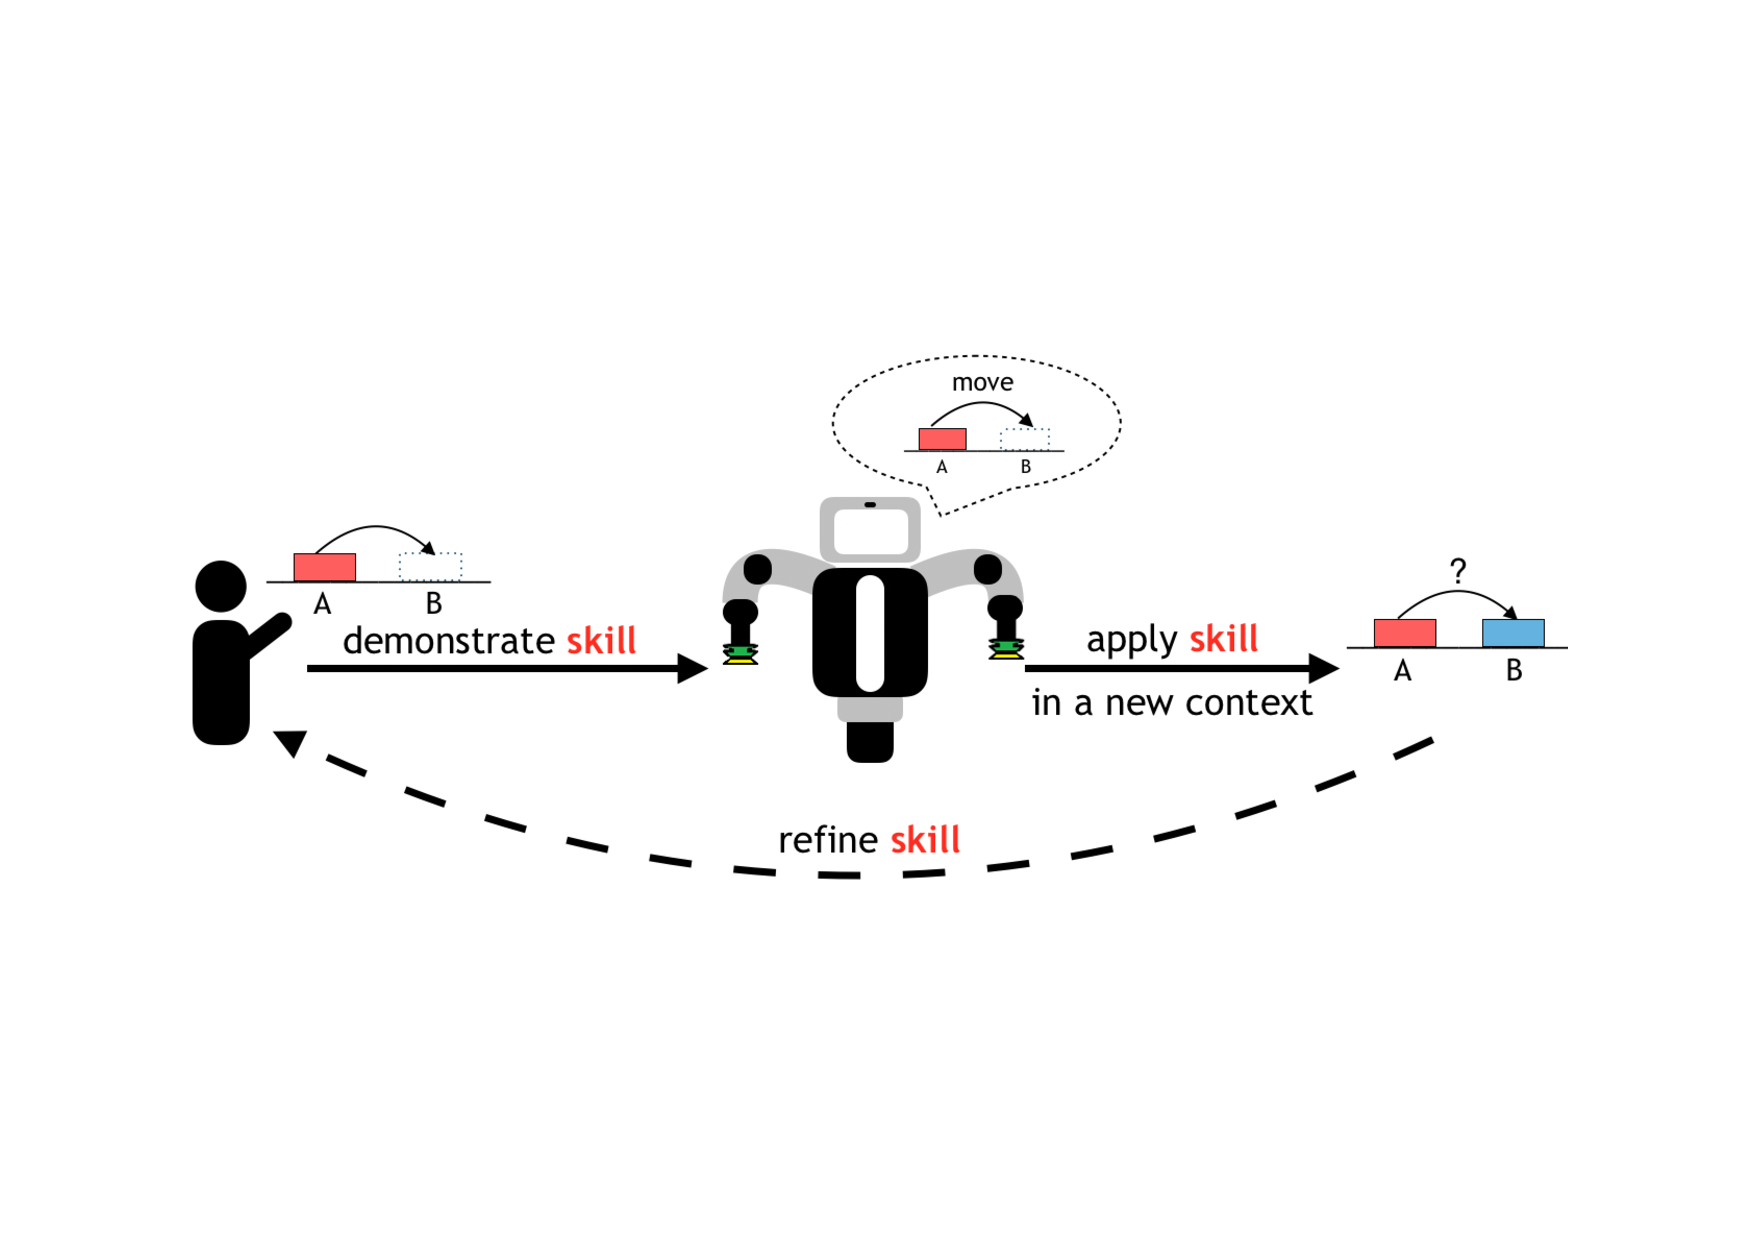
\includegraphics[scale=0.7]{figures/PbD-Overview}
    \caption{PbD Overview}
    \label{fig:Principle Overview}
  \end{figure}

%Besides the advantage of being able to teach the robot tasks without the need to write code, PbD provides a powerful tool to improve learning abilities by reducing the search space of possible solutions.


\subsection{Problem Statement}
Learning object manipulation tasks is considered a hard problem, as the robot has limited knowledge about the world and restricted sensor availability \cite{ekvall2008robot}.
Many PbD algorithms have been proposed in the literature (\cite{argall2009survey}, \cite{billing2010formalism}), but there still remain several challenges that address the suboptimality of demonstrations (\cite{chen2003programing}, \cite{kaiser1995obtaining}) or the lack of comparative user studies (\cite{suay2012practical}).
% teaching full action sequences
The challenge we address in this thesis is that in existing PbD implementations the robot learns an action sequence \cite{EricM.Orendt2016,peppoloni2014ros}, rather than atomic actions that can be reused independently. 
Teaching full action sequences is often complicated and time-consuming, as the robot has to be demonstrated a new sequence, whenever the goal changes.
The user could select task execution plans via a user interface \cite{guerin2015framework}, but ideally, the robot should deduce a task execution plan for a given goal autonomously.

Current approaches only teach the robot an action for manipulating an object, but do not explicitly associate a semantic meaning to it, other than assigning it a name.
If the robot is taught an action's semantic meaning, i.e. the conditions for executing the action, it is provided with the relevant application context and could reuse the action in different contexts.
For example, the robot is taught to pick up an object from an initial position and place it on a goal position.
Conditions for executing this action (e.g. to grab an object only if the gripper is free) are generally neglected during the demonstration.
If the teacher demonstrates a pick-up action to the robot, there is no mention of communicating the conditions for when it can execute the action.

A robot that learns how to arrange items on a desk may have to plan the order of handling differently sized objects in another way than originally demonstrated by the teacher.
Thus, it does not suffice for the robot to replicate the demonstrated movement, but it needs to understand and interpret the teacher's intention so that it can apply the action to different scenarios.

%\section{Problem statement}
Nowadays, non-experts cannot (re-)program robots easily as functionalities are preprogrammed and difficult to modify.
We want to allow non-experts in industrial contexts to program robots using an intuitive and fast method.
We need to consider the limitations: limited resources, lack of programming knowledge and time to train operators.
In this thesis, we want to create a framework that allows robots to solve problems in a goal-oriented way.
In other words, given a user-defined goal, the robot should generate and execute the right action sequence to obtain it.
The user must construct a knowledge base, consisting of a domain model (the environment that the robot interacts with) and all action models required for the robot to accomplish the defined task.

Consider again the example of permutating two objects on the table.
The domain would consist of a table with a finite number of objects and limited positions, as well as actions models consisting of pick, place and move. Possible goals could be to stack the objects by size (similar to the Tower of Hanoi problem \cite{douglas1985metamagical}) or to arrange the objects in a certain order. Our framework should enable the user to teach the robot by demonstration all action models needed, including their relevant preconditions and effects. Once the action models have been created, the inbuilt automated planner can generate an action sequence to achieve any goal within the domain. 

%Hence, we address two common situations, where reprogramming is required: 
%\begin{itemize}
%\item A new subtask needs to be included in the task execution, e.g.
the robot knows how to place objects from any position on the table into a basket, but should additionally rotate them before placing them;
%\item All subtasks are available but the ultimate goal has changed, e.g.
the order of placing the objects has been changed.
%\end{itemize}
